\documentclass[english]{article}

\usepackage{ae,aecompl}
\usepackage[T1]{fontenc}
\usepackage[latin9]{inputenc}
\usepackage{textcomp}
\usepackage{graphicx}
\usepackage{eurosym}
\usepackage[hidelinks]{hyperref}
\usepackage{float}
\usepackage{fancyhdr}
\usepackage{color}
\definecolor{mygreen}{rgb}{0,0.6,0}
\definecolor{mygray}{rgb}{0.5,0.5,0.5}
\definecolor{mymauve}{rgb}{0.58,0,0.82}


\usepackage{listings}
\lstdefinelanguage{alloy}
{
	morekeywords=
					{
							assert, pred, all, no, lone, one, some, check, run,
							but, let, implies, not, iff, in, and, or, set, sig, Int, int,
							if, then, else, exactly, disj, fact, fun, module, abstract,
							extends, open, none, univ, iden, seq, this, Instance, found, No
					},
	sensitive=true,  
	morecomment=[l]//,
	morecomment=[l]{--},
	morecomment=[s]{/*}{*/},
	morestring=[b]",
	numbers=none,
	firstnumber=1,
	numberstyle=\tiny,
	stepnumber=2,
	basicstyle=\scriptsize\ttfamily,
	ndkeywordstyle=\bfseries,
}

\lstset{ %
  backgroundcolor=\color{white},   % choose the background color; you must add \usepackage{color} or \usepackage{xcolor}
  basicstyle=\footnotesize,        % the size of the fonts that are used for the code
  breakatwhitespace=false,         % sets if automatic breaks should only happen at whitespace
  breaklines=true,                 % sets automatic line breaking
  captionpos=b,                    % sets the caption-position to bottom
  commentstyle=\color{mygreen},    % comment style
  deletekeywords={...},            % if you want to delete keywords from the given language
  escapeinside={\%*}{*)},          % if you want to add LaTeX within your code
  extendedchars=true,              % lets you use non-ASCII characters; for 8-bits encodings only, does not work with UTF-8
  frame=single,                    % adds a frame around the code
  keepspaces=true,                 % keeps spaces in text, useful for keeping indentation of code (possibly needs columns=flexible)
  keywordstyle=\color{blue},       % keyword style
  language=alloy,                 % the language of the code
  morekeywords={*,...},            % if you want to add more keywords to the set
  numbers=left,                    % where to put the line-numbers; possible values are (none, left, right)
  numbersep=5pt,                   % how far the line-numbers are from the code
  numberstyle=\tiny\color{mygray}, % the style that is used for the line-numbers
  rulecolor=\color{black},         % if not set, the frame-color may be changed on line-breaks within not-black text (e.g. comments (green here))
  showspaces=false,                % show spaces everywhere adding particular underscores; it overrides 'showstringspaces'
  showstringspaces=false,          % underline spaces within strings only
  showtabs=false,                  % show tabs within strings adding particular underscores
  stepnumber=2,                    % the step between two line-numbers. If it's 1, each line will be numbered
  stringstyle=\color{mymauve},     % string literal style
  tabsize=2,                       % sets default tabsize to 2 spaces
  title=\lstname                   % show the filename of files included with \lstinputlisting; also try caption instead of title
}
\pagestyle{fancy}
\lhead{\powerenjoy RASD}

\newcommand{\carsharing}{\textit {car sharing }}
\newcommand{\powerenjoy}{\textit{PowerEnjoy }}
\newcommand{\registereduser}{\textit {registered user }}
\newcommand{\registeredusers}{\textit {registered users }}
\newcommand{\powerenjoyuser}{\textit{PowerEnjoy User }}
\newcommand{\staff}{\textit{staff }}
\newcommand{\service}{\textit{service }}
\newcommand{\services }{\textit{services }}
\newcommand{\safearea}{\textit{safe area }}
\newcommand{\safeareas}{\textit{safe areas }}
\newcommand{\powergrid}{\textit{power grid }}
\newcommand{\powergrids}{\textit{power grids }}
\newcommand{\reservation}{\textit{reservation }}
\newcommand{\stand}{\textit{stand }}
\newcommand{\rent}{\textit{rent }}
\newcommand{\fieldstaff}{\textit{field staff }}
\newcommand{\resevation}{\textit{reservation }}
\newcommand{\stopover}{\textit{stopover }}
\newcommand{\personalpin}{\textit{personal pin }}
\newcommand{\guest}{\textit{guest }}
\newcommand{\thirdparty}{\textit{third party developer}}
\usepackage{tabto}
\usepackage{verbatim}
\usepackage{etoolbox}
\usepackage[table]{xcolor}
\usepackage{booktabs}
\usepackage{wasysym}
\usepackage{multirow}

\begin{comment} some new commands and environments to painlessly handle requirements, goals and domain assumptions listing \end{comment}
\newenvironment{goals}
		{
			\newcounter{goalId}
			\newcommand{\goal}[1]{ 
				\stepcounter{goalId} 
				\hypertarget{G\arabic{goalId}}{
					\item[
						 G.\arabic{goalId}
					]{ ##1 }
				}
			}
			\begin{description}
		}
		{
			\end{description}
		}

\newenvironment{domainassumptions}
	{
		\newcounter{domainassumptionId}
		\newcommand{\domainassumption}[1]{ 
			\stepcounter{domainassumptionId} 
			\item[D.\arabic{domainassumptionId}]{##1}
			}
		\begin{description}
	}
	{
		\end{description}
	}

\newcounter{reqId}
\newenvironment{requirementsgroup}
		{
			\newcommand{\req}[1]{ 
				\stepcounter{reqId} 
				\hypertarget{R\arabic{reqId}}{
					\item[
						 R.\arabic{reqId}
					]{ ##1 }
				}
			}
			\begin{description}
		}
		{
			\end{description}
		}
\newcommand{\goalref}[1]{  \hyperlink{G#1}{G.#1} }
\newcommand{\reqref}[1]{  \hyperlink{R#1}{R.#1} }

\makeatletter
\usepackage{babel}


\makeatother

\usepackage{babel}
\begin{document}
\begin{figure}
	\centering
	
\includegraphics[scale=0.5]{logo.pdf} 
\end{figure}


\title{\powerenjoy\\
 Requirement Analysis and Specification Document\\
}

\date{A.A 2016/2017}

\author{Erba Alessandro\\
 Leveni Filippo\\
 Lodi Luca}

\maketitle
\pagebreak{}

\tableofcontents{} \pagebreak{}

\section{Introduction}
	\subsection{Purpose}
	
		The purpose of our team is to project \powerenjoy, which is  a platform that will be used to manage a \carsharing \service  in the city area.\\
 		The platform will allow clients to find and reserve electric cars using smart devices (In Section 5 these devices are described), and it will also manage the communication of the emergency situations to the proper \staff.\\
  		Furthermore, a particular \powerenjoy feature is the application of certain discounts to its users.\\
 		 \tab \tab This document aims to describe the high-level functionalities that will be offered by \powerenjoy \service. The RASD is intended to be viewed by the stakeholders , that will evaluate the correctness of any assumption and decision in this document.
  
 \subsection{Scope}
 
  %PowerEnJoy would introduce an ecological way to travel within the city area. Uniform distribution of cars in the city is a significant target.
%  \par The cars are electric. And h Through this interface   is possible to communicate with the system (e.g. to call emergency \staff).\\
%   \tab \tab Users can choose and reserve a car through a mobile app. The system answers to the request by showing the    time left to the expiration of the \reservation.\\
 %  The \staff is divided in three categories:\\
 %   - Field \staff\\
 %   - Emergency \staff\\
 %   - Management \staff\\
  % \tab \tab Field \staff use the mobile application to inform the system about their availability and to confirm that they are    going to take care of a certain call (e.g. retrieve a broken car, move a vehicle with a low battery or to ensure the uniform    distribution in the city, etc...).\\
%   \tab \tab Emergency \staff use the mobile application to answer customers calls and to take care of special situations (e.g. car % accident).\\
%   \tab \tab Management \staff use the mobile application to handle the \service (e.g. set the \safeareas, fares, discounts,     etc...).\\
%   \tab \tab The system guarantees a uniform distribution of cars in the city. The way in which this is guaranteed is explained later in this document.   \\
%   \tab \tab A user can take advantage of the "Money saving" option selecting it on the integrated interface in the car. After    that he/she can input his/her final destination and the system provides information about the station where to leave the car to get a discount. This destination is determined to ensure the uniform distribution of cars and depends both on the destination of the user and on the availability of power plugs at the selected station.

PowerEnJoy service is a car sharing service. Its aim is to develop a new way of car sharing.
three crucial and innovative points of the service:

\begin{itemize}
	\item Electric cars.
	\item Uniform distribution of cars, in order to easily find a car near the user position.
	\item Discount policies for users eco-friendly behaviors.
\end{itemize}

Through our analysis we have figured out how the system could be organized.
We have identified Actors and situations that can be useful to manage the system.

	
	\subsection{Goals}

	We have selected a list of objectives that we think \powerenjoy  has to reach:
	\begin{goals}
		
		\begin{comment} drivers for PowerEnjoy's success \end{comment}
		\goal{ To allow user to simply access to the \powerenjoy services. }
		\goal{ To guarantee an higher  probability of finding a car, compared to other car sharing services. }
		\goal{ To guarantee an efficient maintenance and recharge process of the cars, oriented to favourite their fairly distribution over the territory. }
		\begin{comment} user's goals \end{comment}
		\goal{ To allow users to make a reservation for a car in advance, and to cancel a reservation by its expiration time. }
		\goal{  To transparently charge the user for the service, minimizing its interaction with payment interfaces. }
		\goal{  To allow users to drive cars, minimizing their efforts for finding safe areas where to park.}
		\goal{ To encourage users' virtuous behaviour  in relation to service's fairness. }
		\begin{comment} service efficiency goals \end{comment}
		\goal{ To create a system that gives the possibility to be monitored and administrated by \powerenjoy's authorized personal. }
		\goal{  To empower the authorized personal in order to be able to quickly react to emergencies, potentially dangerous situations and users' requests for help, in best interest of users' safety.}
		\goal{ To create a system that provides a programmable interface, in order reduce the costs of further enhancements / maintenance to the system exploiting internal personal or third party developers.}
		
		% \goal{ . }

	\end{goals}


	\subsection{Domain Assumptions }

	We suppose that the following conditions hold in the analysed world:
	\begin{domainassumptions}

		\domainassumption{ The geographical area covered by the service is included in the coverage area of most common mobile communication technologies (3g, 4g) offered by main telecommunications companies. }

		\domainassumption{ Only correctly registered users can access the functionalities provided by the system. }
		\domainassumption{ Users will not park cars in position not covered by GPS signal (such as underground parking slots). }

		\domainassumption{ Cars are able to send diagnostic for the maintenance process in addition to real-time telemetry about speed and status of the battery.  }
		\domainassumption{ Cars can be selectively remotely locked, unlocked, powered on and powered off by authorized personal. }
		\domainassumption{ Cars periodically notify the system of their position, in case of accident / failure the notification process stops. }
		\domainassumption{ Cars are provided with an hand-free communication set that can be remotely activated. }

		\domainassumption{ Both user's and cars' GPS position can't be faked by any mean (e.g: GPS spoofing). }

		\domainassumption{ Each plug in charge stations is capable to be remotely  enabled/disabled for the charge of cars. }
		
		%\domainassumption{ . }

	\end{domainassumptions}

	\subsection{Glossary}
		\label{sec:Glossary}
		\subsubsection{Car Sharing}
			\carsharing is a model of car rental where people rent cars for short periods of time, often by the hour.
		\subsubsection{PowerEnJoy}
			\powerenjoy is the \carsharing brand object of this document.
		\subsubsection{Guest User}
			A \guest is a person not logged in to the system.
		\subsubsection{Registered User} 
			A \registereduser is a person registered to \powerenjoy.
		\subsubsection{PowerEnJoy User}
			A \powerenjoyuser is a \registereduser can access to the \carsharing through his smart-phone.
		\subsubsection{Staff}
			\staff is the set of people that are \registereduser  but can perform special operations. They are divided in three different categories.
			\begin{itemize}
				\item {Field \staff}
				\begin{itemize}
				\item They own a passepartout for cars that has all kind of issues, for example they can manage cars with low battery.
				\end{itemize}
				\item{Emergency \staff}
				\begin{itemize}
				\item They manage users issues. They are available to communicate with users.
				\end{itemize}
				\item{Management \staff}
				\begin{itemize}
				\item They manage the system, for example they can change system parameters. They can add new \safeareas, modify \carsharing prices.
				\end{itemize}
			\end{itemize}
		\subsubsection{Third Party Developer}
			\thirdparty is a person that can fulfill operations on \powerenjoy system via API.
		\subsubsection{Service}
			The \service is the group of actions that a \powerenjoyuser can fulfill trough the mobile.	
		\subsubsection {Safe Area}
			A \safearea is a  geographical place\footnote{defined by a set of GPS positions} on the map in which parking is allowed. \safearea are saved into the system. A \powerenjoyuser can end a \carsharing parking his car only in safe areas.
	\subsubsection{Power Grid}
		A \powergrid is the station that charge the battery of an electric car. All \powergrid are displayed in the map on-board \powerenjoy cars. Each \powergrid is in a \safearea. A \powerenjoyuser who plugs his car into a \powergrid receives the discount expected within \powerenjoy rules.
	\subsubsection{Reservation}
		A \resevation is the possibility that a \powerenjoyuser has to book a car at the latest for one hour.
	\subsubsection{Stopover}
		A \stopover is the possibility that a \powerenjoyuser has to pause his \carsharing. During a \stopover the \powerenjoyuser can leave the car, than he can re-unlock it through his smart-phone.
	\subsubsection{Personal  Personal Identification Number (pin)}
		 \personalpin is a number of 5 digits that the user inserts on the car screen to enable driving commands.

\subsection{Further Developments}
	We think that one of the most important things is to release a \service that can be extended and improved. It's trivial that a \service like this must be able to be changed and updated.
	For this purpose we will develop a system open to new extensions. \\
	Here we provide a series of possible extensions that could be necessary in the future.
	E.g.:
	\begin{itemize}
		\item New kind of discount policies can be introduced to the system, for example discounts for new types of users. 
		\item New system policies may be necessary, for example new \carsharing conditions.
		\item New kind of vehicles can be introduced, for example electric scooters and electric bikes.
		\item Support to new payment methods, for example Paypal\textregistered, NFC\footnote{Near Field Communication; NFC devices are used in contactless payment systems, similar to those used in credit cards and electronic ticket smartcards and allow mobile payment to replace/supplement these systems. \href{https://en.wikipedia.org/wiki/Near_field_communication}{NFC on Wikipedia}}.
		\item Develop new \service in order to increase the user experience, for example it may be useful to allow communication among users in order to share a car ride and save money.
	\end{itemize}
	\subsection{Used Tools}
	\begin{itemize}
		\item \LaTeX\\
		\item GitHub\\
		\item Astah\\
	\end{itemize}
\section{Specific Requirements}
	\subsection{Functional Requirements}
	
	\subsubsection{Guest users}
	The system must give guest users the possibility to:
	\begin{requirementsgroup}
		\req{ to register to the system by providing their credentials, payment information and required documents.
			\begin{itemize}
				\item{credentials must be unique among previously registered users }
				\item{documents and payment information must be verified in order to successfully create an account.}
			\end{itemize}
		 }
		\req{ to receive back password (for login) and pin code (to power on cars) in case off successful registration . }
	\end{requirementsgroup}	
	
	
	\subsubsection{Registered users}
	Registered users must be allowed to:
	\begin{requirementsgroup}
		\req{  to log-in as \powerenjoy users or field/emergency/management staff user. }
		\req{  to reset the password.}
		\req{  to modify account data. }
	\end{requirementsgroup}
	
	\subsubsection{ \powerenjoy users }
	They are registered users, so they are subject to the same requirements, moreover the system must guarantee them:
	\begin{requirementsgroup}
		 \req { to find the locations of available cars within a certain distance from their current location or from a specified address.
			\begin{itemize}
				\item{information are provided regarding the cars' estimated autonomy in kilometers }
			\end{itemize}
		 }
		 \req { to reserve a single car, among the available ones, for up to one hour before picking it up (by unlocking the car).}
		 \req { to cancel the reservation before it's expiration
			\begin{itemize}
				\item{paying a cost proportional to the reservation time }
				\item{the minimum amount is relative to a quarter of an hour}
			\end{itemize}
		}
		 \req { to be charged of a fee (1\euro) whether the reserved car is not picked\textendash up within one hour from the reservation.
			\begin{itemize}
				\item{the car must be tagged as available again }
				\item{the reservation expires}
			\end{itemize}
		 }

		 \req { to rent a car (reserved or available), specifically:
			\begin{itemize}
				\item { to unlock a reserved car when it is within a certain distance (threshold) from the car }
				\item { to be charged for a given amount of money per minute as soon as the car is unlocked. } 
			 	\item { to be notified of the current fare through a screen on the car. }
			 	\item { to stop being charged as soon as the car is parked in a safe area and he exits the car (that is automatically locked) }
			\end{itemize}
		}
		 
		 \req { to be excluded from the fruition of \powerenjoy services whether the payment is unable to complete, until all pending payment are performed.  }

		 \req { to be applied a discount of 10\% on the last ride, whether it brings at least two other passengers onto the car. }
		 \req { to be applied a discount of 20\% on the last ride, whether the car is left with more than 50\% of the battery's charge. }
		 \req { to be applied a discount of 30\% on the last ride, whether it takes care of plugging-in the car to the charge station. }
		 \req { to be applied an overcharge of 30\% on the last ride, whether the car is left farer than 3 KM from the nearest charge station or with less than 20\% of the battery's charge. }
		 \req { to enable the money saving option in order to get the discount described above [\reqref{14}], specifically:
			\begin{itemize}
				\item { to input a destination }
				\item { to be shown information about where to park the car (within 1km from entered destination) } 
			\end{itemize}
		}

		\req { to be notified of changes in the service policies
			\begin{itemize}
				\item { different fares }
				\item { updated terms of services } 
			\end{itemize}
		}
	\end{requirementsgroup}	

	\subsubsection{ Field staff users }
	They are registered users, so they are subject to the same requirements, moreover the system must help them:
	\begin{requirementsgroup}
		\req{ to be notified of relocation/maintenance requests for cars }
		\req{  to relocate an assigned car:
			\begin{itemize}
				\item{locate assigned car }
				\item{unlock assigned car}
				\item{check diagnostic of assigned car}
				\item{power on assigned car}
				\item{enable / disable power plugs}
				\item{lock assigned car}
				\item{locate maintenance facility}
			\end{itemize}
		 }
		\req{ to ask for special equipment (e.g: tow truck) or additional field staff help after evaluating the situation. }
	\end{requirementsgroup}

	\subsubsection{ Management staff users }
	They are registered users, so they are subject to the same requirements, moreover the system must empower them:
	\begin{requirementsgroup}
		 \req { to configure the list of available safe areas and power plugs over the service covered area. }
		 \req { to configure the list of cars available for the service }
		 \req { to configure service policies: 
			\begin{itemize}
				\item{update existing service's fares}
				\item{introducing new service's fares}
				\item{update discounts}
				\item{introducing new discounts}
				\item{update the terms of the service}
			\end{itemize}
		  }
		 \req { to manage personnel's accounts:
			\begin{itemize}
				\item{create}
				\item{delete}
				\item{modify}
			\end{itemize}
			for:
			\begin{itemize}
				\item{field staff user}
				\item{emergency staff user}
				\item{management staff user}
			\end{itemize}
		}
		 \req { to handle exceptional cases of unpaid rents:
			\begin{itemize}
				\item{check pending payment status.}
				\item{re-enable \powerenjoy users to the service.}
			\end{itemize}
		 }
	\end{requirementsgroup}

	\subsubsection{ Emergency staff users }
	They are registered users, so they are subject to the same requirements, moreover the system must empower them:
	\begin{requirementsgroup}
		\req{ to be promptly notified of potentially dangerous situations / emergencies: 
			\begin{itemize}
				\item{cars malfunctioning during a rent}
				\item{car accidents}
				\item{cars with empty battery not parked in safe areas}
			\end{itemize}
		 }
		\req{ to be promptly notified of \powerenjoy users' help request.  }
		\req{ to have an overview regarding the state and location of:
			\begin{itemize}
				\item{cars}
				\item{power plugs}
				\item{current rents}
				\item{reservation}
				\item{field staff users} 
			\end{itemize}
		}
		\req{ to perform actions to resolve issue:
			\begin{itemize}
				\item{cancel a \powerenjoy user's reservation}
				\item{recover a \powerenjoy user's pin code}
				\item{unlock / lock rented car}
				\item{set a car as available / unavailable }
				\item{speak with user on rented cars through installed hands-free communication set} 
				\item{assign a field staff user to relocate a car with priority}
				\item{notify appropriate authorities of a car accident (first-aid, fire-fighters, police, insurance company ...) }
			\end{itemize}
		 }
		\req { to dispatch the issue to administration staff users.}
		
	\end{requirementsgroup}

	\subsubsection{ Third party developers }
	The system should permit third party developers:
	\begin{requirementsgroup}
		\req{ to access all the functionalities of a \powerenjoy users through a set of public APIs (provided the user gave the consensus).}
		\req{ to register new \powerenjoy users through a set of public APIs. }
	\end{requirementsgroup}
	
	\subsubsection{ Requirement - Goals mapping}
	
	%\rowcolors{3}{gray!25}{white!50}
	\begin{table}[H]
	\newcommand{\C}{\CheckedBox}
	\newcommand{\U}{\Square}
	\centering
	$\begin{array}{ c c *{4}{c}  *{4}{c}  *{2}{c}  }
	\toprule
	\emph{Actor} & \emph{Req.}  & \multicolumn{10}{c}{\emph{Goal} } \\
	\midrule
	&&\goalref{1} & \goalref{2} & \goalref{3} & \goalref{4} & \goalref{5} & \goalref{6} & \goalref{7} & \goalref{8} & \goalref{9} & \goalref{10}\\
	\multirow{2}{*}{Guest user} 
	& \reqref{1} & \C & \U & \U & \U & \U & \U & \U & \U & \U & \U  \\
	& \reqref{2} & \C & \U & \U & \U & \U & \U & \U & \U & \U & \U  \\
	\hline
	\multirow{3}{*}{Registered user} 
	& \reqref{3} & \C & \U & \U & \U & \U & \U & \U & \U & \U & \U  \\
	& \reqref{4} & \C & \U & \U & \U & \U & \U & \U & \U & \U & \U  \\
	& \reqref{5} & \C & \U & \U & \U & \U & \U & \U & \U & \U & \U  \\
	\hline
	\multirow{12}{*}{\powerenjoy user} 
	& \reqref{6} & \U & \C & \U & \U & \U & \U & \U & \U & \U & \U  \\
	& \reqref{7} & \U & \U & \U & \U & \U & \U & \U & \U & \U & \U  \\
	& \reqref{8} & \U & \U & \U & \U & \U & \U & \U & \U & \U & \U  \\
	& \reqref{9} & \U & \U & \U & \U & \U & \U & \U & \U & \U & \U  \\
	& \reqref{10} & \U & \U & \U & \U & \U & \U & \U & \U & \U & \U  \\
	& \reqref{11} & \U & \U & \U & \U & \U & \U & \U & \U & \U & \U  \\
	& \reqref{12} & \U & \U & \U & \U & \U & \U & \U & \U & \U & \U  \\
	& \reqref{13} & \U & \U & \U & \U & \U & \U & \U & \U & \U & \U  \\
	& \reqref{14} & \U & \U & \U & \U & \U & \U & \U & \U & \U & \U  \\
	& \reqref{15} & \U & \U & \U & \U & \U & \U & \U & \U & \U & \U  \\
	& \reqref{16} & \U & \C & \U & \U & \U & \U & \U & \U & \U & \U  \\
	& \reqref{17} & \U & \U & \U & \U & \U & \U & \U & \U & \U & \U  \\
	\hline
	\multirow{3}{*}{Field staff user} 
	& \reqref{18} & \U & \U & \U & \U & \U & \U & \U & \U & \U & \U  \\
	& \reqref{19} & \U & \C & \U & \U & \U & \U & \U & \U & \U & \U  \\
	& \reqref{20} & \U & \U & \U & \U & \U & \U & \U & \U & \U & \U  \\
	\hline
	\multirow{5}{*}{Management staff user} 
	& \reqref{21} & \U & \U & \U & \U & \U & \U & \U & \U & \U & \U  \\
	& \reqref{22} & \U & \U & \U & \U & \U & \U & \U & \U & \U & \U  \\
	& \reqref{23} & \U & \U & \U & \U & \U & \U & \U & \U & \U & \U  \\
	& \reqref{24} & \U & \U & \U & \U & \U & \U & \U & \U & \U & \U  \\
	& \reqref{25} & \U & \U & \U & \U & \U & \U & \U & \U & \U & \U  \\
	\hline
	\multirow{5}{*}{Emergency staff user} 
	& \reqref{26} & \U & \U & \U & \U & \U & \U & \U & \U & \U & \U  \\
	& \reqref{27} & \U & \U & \U & \U & \U & \U & \U & \U & \U & \U  \\
	& \reqref{28} & \U & \U & \U & \U & \U & \U & \U & \U & \U & \U  \\
	& \reqref{29} & \U & \U & \U & \U & \U & \U & \U & \U & \U & \U  \\
	& \reqref{30} & \U & \U & \U & \U & \U & \U & \U & \U & \U & \U  \\
	\hline
	\multirow{2}{*}{Third party developer} & \reqref{31} & \U & \U & \U & \U & \U & \U & \U & \U & \U & \U  \\
	& \reqref{32} & \U & \U & \U & \U & \U & \U & \U & \U & \U & \U  \\
	%\bottomrule
	\end{array}$
	\end{table}
	
\subsubsection{Functional Requirements Priorities}
Among the Functional requirements introduced in this section, we identify an importance priority list from the Company Point of View.
\begin{enumerate}
	\item \textbf{PowerEnJoy User Requirements}: it's trivial that this is the core for the Company, provide the service.
	\item \textbf{Staff Requirements}: the backend is very important in order to guarantee a trustful service
	\item \textbf{Third Party Development Requirement}: despite we believe that it is very important the integration in other systems, it's priority it's the lower compared to the others
\end{enumerate}

	\subsection{Non Functional Requirements}
		\subsubsection{Usability}
		The application must be easy to use from the user point of view. The user interface should respect the \href{https://www.iso.org/obp/ui/#iso:std:iso:tr:16982:ed-1:v1:en}{ISO/TR 16982:2002 standard.} 
During the development of the user interface will be purposed some sample tests to some people in order to answer to these points.
	\begin{itemize}
		\item Learnability: How easy is it for users to accomplish basic tasks the first time they encounter the design?
		\item Efficiency: Once users have learned the design, how quickly can they perform tasks?
		\item Memorability: When users return to the design after a period of not using it, how easily can they re-establish proficiency?
		\item Errors: How many errors do users make, how severe are these errors, and how easily can they recover from the errors?
		\item Satisfaction: How pleasant is it to use the design?
	\end{itemize}
		\subsubsection{Availability, Reliability, Fault Tolerance, Disaster Recovery}
		Every user should be able to start a new ride in every moment of the day. Ideally the whole  infrastructure must be able to serve \registereduser 24/7. If the system goes down, the \powerenjoy company will loose money. \par It is trivial that our purpose is to guarantee the best reliability\footnote{Here we refer to the literal meaning, how accurate or able to be trusted someone or something is considered to be}.\par In order to pursue this objective our system architecture must be developed guaranteeing:
		\begin{itemize}
			\item Availability: at least 99.99\% (Downtime: approx 8.66 seconds per day, 52,56 minute per year) for the back end, 99.9\% (Downtime:1.44 minute per day) for the UI.
			\item Reliability: at least 2 month between failures.
			\item Fault Tolerance: the probability of a failure that makes the system unusable is less than 0.001\%.
			\item Disaster Recovery: All Informations about users, cars, \safearea must be recoverable after disaster situation with a probability of 99.999\%.
		\end{itemize}
		\subsubsection{Privacy}
		Every country where the system is released has its own laws in matter of Privacy and respect of personal data. The system must be developed in the respect of these norms.\par Let's take for example that the system operates in Italy. Here is in force the D.Lgs. 196/2003 \href{http://www.camera.it/parlam/leggi/deleghe/03196dl.htm}{(D.Lgs. on www.camera.it website)} about personal data protection. The system must respect the local law, otherwise the company will be penally prosecutable.
		\subsubsection{Security}
		The system security provides secure communication among users and serves and guarantees the protection of data from malicious agents. In order to guarantee security the system must be conformed to the ISO 27001:2013 "Information technology - Security techniques - Information security management systems - Requirements" \footnote{\href{https://en.wikipedia.org/wiki/ISO/IEC_27001:2013}{ISO 27001:2013 on Wikipedia}}
		\subsubsection{Portability}
		The software should work on at least the 90\% of commercial devices described the paragraph about External interface. Furthermore the system source code must be portable from a platform to another for at least the 75\%.		
		
		\subsubsection{Money Saving Car distribution}
		As said in the Assignments document, the money saving option guarantees uniform distribution of cars in the \safearea.\par In order to do that the system will be able to drive \registereduser to the correct \powergrid, if money saving is activated. Each city covered by the service will be divided in concentric circles that form circular crowns, each circular crown is divided in slices, called City Zones. Each City Zone has its own frequency of picking up cars. This frequency is seen as a weight in the map. The weight indicates proportionally the optimal number of cars that should be available in that zone. So, given the destination of the \registereduser, the system can calculate the best solution for the user.
The system will provide solutions that are no more far than 1km from the selected destination.
This allocation method is also used from \fieldstaff in order to re-allocate cars that were under maintenance.
		\noindent
		\begin{figure}[H]
\centering
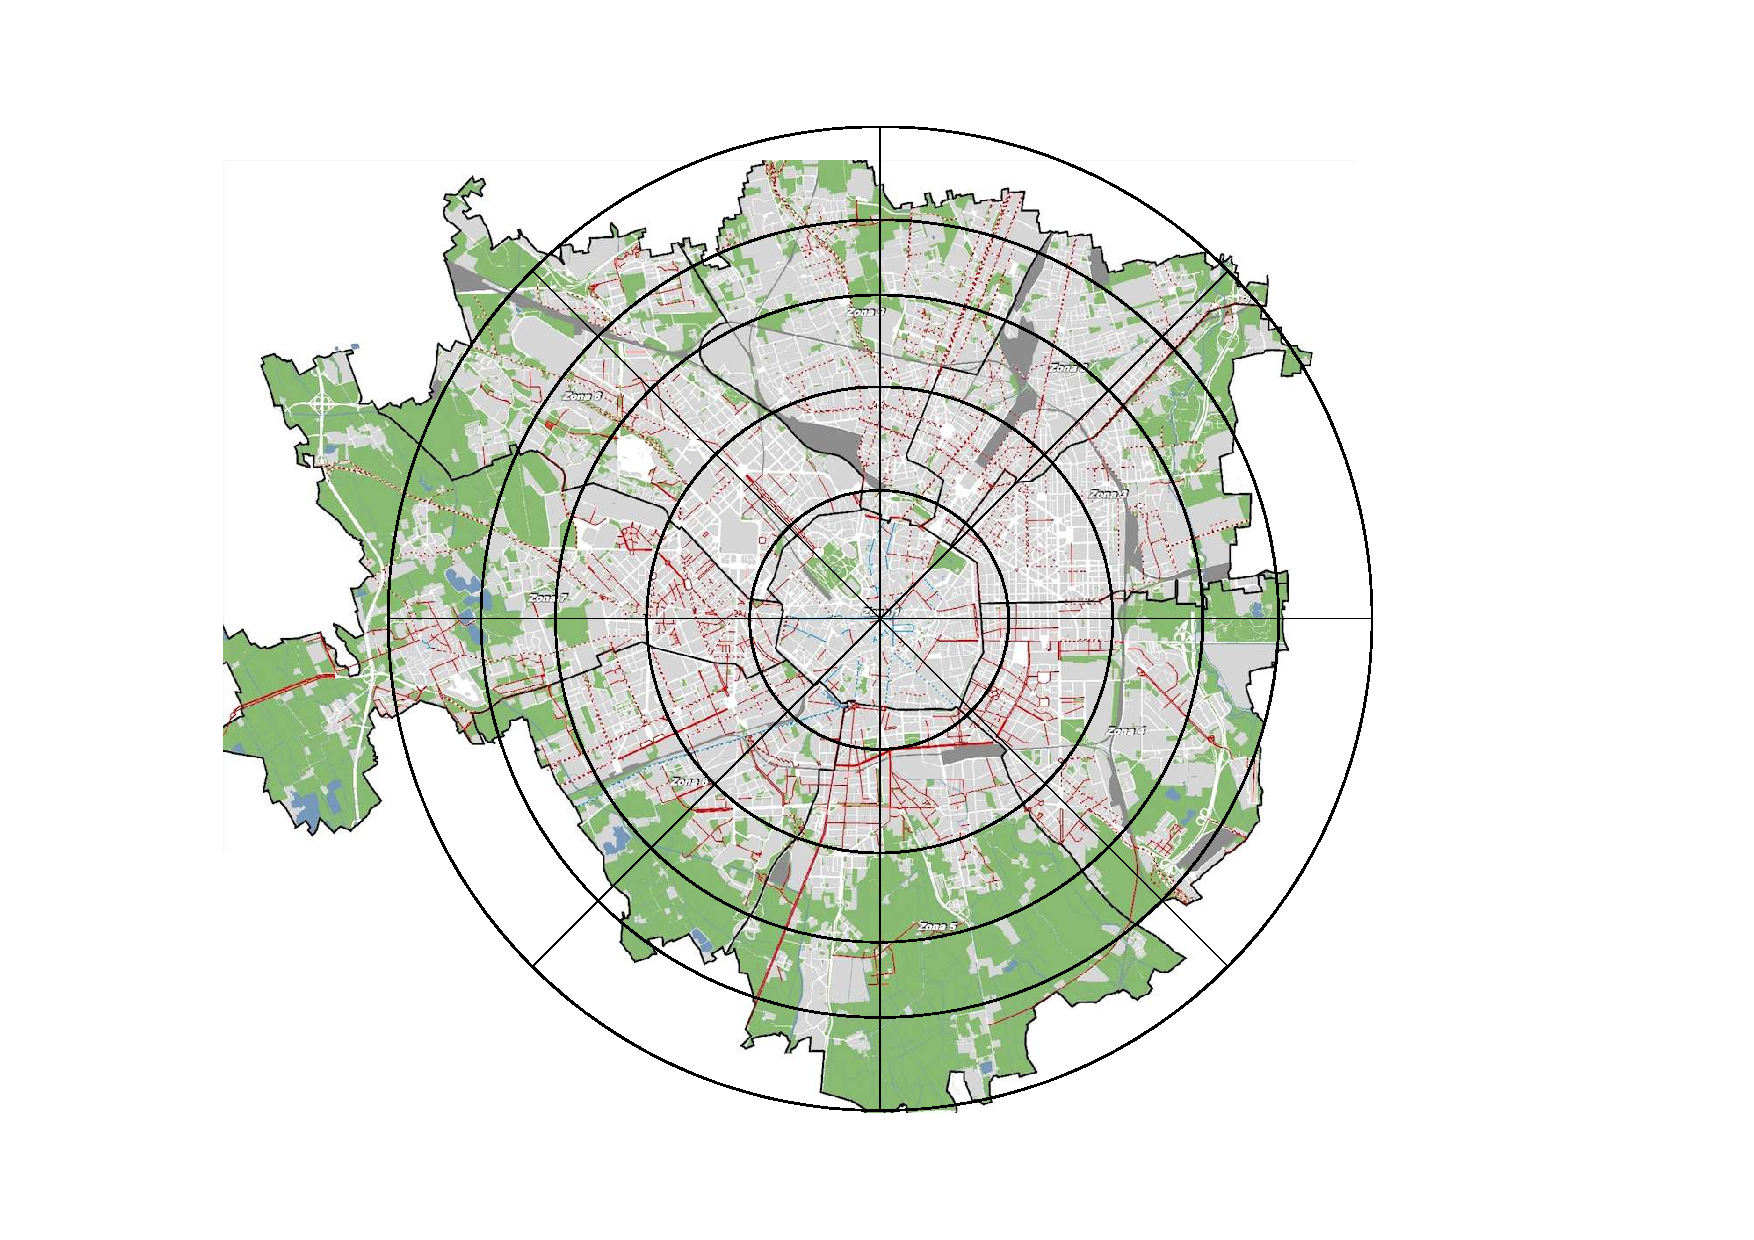
\includegraphics[scale=0.4]{mappazone.pdf}% "%" necessario

\caption{City Zones Map division}
\end{figure}
		

		

		\subsubsection{Application Programming Interface}
		In order to extend its functionalities the system shall provide an programmable interface. That interface represents a way for programmers to create own application which can interact with \powerenjoy. For example our system must be integrable in a car sharing aggregator. So an user using a third party application must be able to reserve its \powerenjoy.
		

\section{Scenarios Identifying}
	To allow you to better understand the behaviour of this service here we present some possible situations.
	\subsection{Scenario 1}
		Alessandro is planning his weekend. It's his best friend's birthday party and he has to reach a place not covered by public transportation. Alessandro decides to subscribe to the new \powerenjoy \service. He downloads the application on his smartphone, opens the app and clicks on the Sing Up menu. He provides all the information needed to join the \service. In order to do that he sends a scan of his driving license and fills an electronic form containing his personal info (personal details, payment info). Finally he agrees to \service's	"Terms and Conditions'' .
		Now he is waiting for an acknowledgement of registration. After a while he receives an email reporting his successfully subscription to the \service. Alessandro can now Log In in the application as a \registereduser.
	\subsection{Scenario 2}
		Ariana feels smart, last week she has rent a \powerenjoy but she has run out of money in her prepaid card, so the system has locked her account. She owns 2 different prepaid credit cards and she tries to re-subscribe to the \service without settle her debt. Ariana provides all the information for subscribing to the \service and sends it. Her application request is denied.
	\subsection{Scenario 3}
		It's Saturday night and Alessandro is a newbie of \powerenjoy \service, he tries to reserve his car, he log in in the app and turns on the GPS of his smartphone. In a few seconds a map appears on the screen. Here are displayed all the available cars around him. Clicking on a car he can see it's autonomy. He chooses the nearest car to his house and reserves it clicking on the ``Reserve Now'' button. From this moment he has an hour before it's \reservation expires. He gets ready for the night and than walks to the car. Once arrived he opens the 	\powerenjoy app and goes to the ``Here I am'' menu. The system checks Alessandro's GPS Position and if he is close enough to the car unlocks it. Alessandro is very happy and gets in the car.
	\subsection{Scenario 4}
		It's Monday morning and Alice is getting ready for her work day. Alice is a \registereduser of \powerenjoy . She is late and won't take the subway today. She reserves a car near her apartment. While she is getting ready for the day, she receives a call from Melissa. Melissa is an Alice working colleague. Melissa is going to pick Alice up. Alice cancels hers \reservation and pays a fee of 0.25\euro because it is passed less than a quarter of an hour from his \reservation time.
	\subsection{Scenario 5}
		Marcus has to carry his son Mario to school. He reserves a \powerenjoy. While they are going downstairs Mario falls down. He loses consciousness and Marcus calls an Ambulance. In this situation Marcus completely forgets to cancel his \reservation, so after an hour 1\euro is charged	on his credit card.
	\subsection{Scenario 6}
		Antony is moving in the subway from Duomo to Sesto Primo Maggio Fs. It's Friday 21th of October and in Sesto Primo Maggio Fs there are not trains to reach Lissone because there is an usual Trenord strike. Fortunately he is a \powerenjoy user. Antony Logs In in the app and selects the manual input car research. Typing on his smartphone ``Sesto San Giovanni'' he easily checks all the available  cars. He chooses a car and reserves it. He is very happy because the "Money Saving Option'' guarantees him an high probable possibility to find a car in each \powerenjoy \safearea. Once in Sesto San Giovanni he unlocks his car while all the other commuter can only hope to reach their home within the day after.
	\subsection{Scenario 7}
		It's raining. Filippo is going towards the \powerenjoy car just reserved when he meets Alessandro and Luca, two his classmates. They have to go home, Filippo offers to give a lift to both for the station and they accept. Once into the car, the system notes that there is two passengers. Arrived at the station Filippo stops the car and his friends leave the vehicle. At this time the system store on its memory that on that stretch of road travelled it will have to apply the discount of 10\%.
	\subsection{Scenario 8}
		Andrew has to carry his mother to the airport but remembers that his car is being repaired. He thinks that the best choice is to reserve a car with the \powerenjoy app. After that they go towards the vehicle and, once reached it, Andrew helps his mother to load the heavy suitcase in the back seat. Now everything is ready to go. On the way by the airport on the screen of the car appears a message that explain to the driver that he finished the money on his credit card, so he can finish this trip but his account will be blocked until he will pay the debts towards the company. Arrived at the airport the mother goes out from the car with her suitcase and says goodbye to her son. Once at home Andrew has to pay the full rent because the system notice that the passenger is only one.
	\subsection{Scenario 9}
		Paul is late for his first day of teaching. Go by foot will not allow him to arrive on time. He decides to reserve a car with his \powerenjoy app. He opens it and checks the available cars. Unfortunately he notices that the only nearby car have 15\% of battery full and the workplace is 4KM from the nearest \powergrid station, outside a \safearea. The workplace is just 10 minutes by car from its position and the time is running out, so 	he reserves it. Left the \safearea, the car advice Paul by the screen that he should 	park in a \safearea, otherwise will be charged recovery costs. He's too much late and ignores the advice. The system will charge 30\% more on this ride because the car is left with less 20\% of the battery's charge and at more that 3KM from the nearest \powergrid station, furthermore Paul will has to pay recovery costs.
	\subsection{Scenario 10}
		Rodolfo has to meet her parents in their downtown manor. He could go by feet but it's a very cold winter day and prefers to reserve a warmer \powerenjoy car. Looking at the cars around him, luckily notices that the nearest car have the battery completely charge! He is clever and kind, so decide not to go directly to his parent's house but to reach the closest station to it in order to plug the car into the \powergrid. Rodolfo reaches the car, get in and starts driving. Arrived at the station, the car's battery level is 90\%. For this journey he will receive a total of 50\% discount: 20\% from the level of the battery ( more than 50\% ) and 30\% from his kindness ( car plugged into a \powergrid ). A very lucky day for Rodolfo!
	\subsection{Scenario 11}
		Amelia is a good mother and be careful to save money for her family, in fact she went to the supermarket by foot. After buying the necessary things for the house, she notices that the bags are too heavy to walk back. She remembers that she is subscribed to the \powerenjoy \service. She logs in the app, reserves a car. Than she picks up the car, selects the destination and chooses the ``money saving option''. Although this unforeseen she can save some money. The system computes the destination in order to get the discount. Once arrived to the destination she locks the car and plugs it into the \powergrid. The system applies a discount of 30\% on her ride.
	\subsection{Scenario 12}
		John is going to the gym using the \powerenjoy \service, when he notices that the car's battery level is critically low, but he decides to go on without takes care of it. At certain point the car informs John that he should go near the roadside because the car will stops shortly. John is a bully and decides to ignore the warning. Taking care of the user's safety the car stops as expected, but John is in the middle of the road! Never having been in a similar situation he decides to call the assistance using the embedded screen on the car. An operator takes the call and explains John that a field \staff is coming on site and until the car is not parked safely he will continue to pay. A very expensive day for our John.		
	
\section{UML Models And Use Cases}
	\subsection{Use Cases Diagram}
	\noindent
	\makebox[\textwidth]{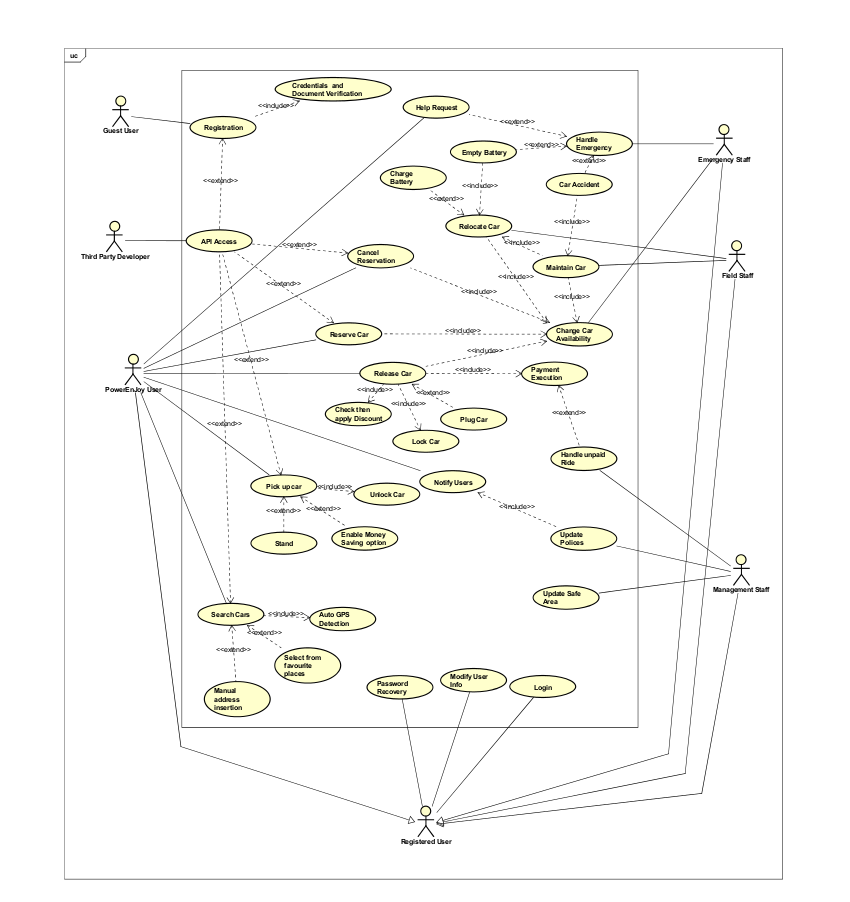
\includegraphics[scale=0.85]{usecase.pdf} }%



	\subsection{Actors Identifying}
		\noindent
		\makebox[\textwidth]{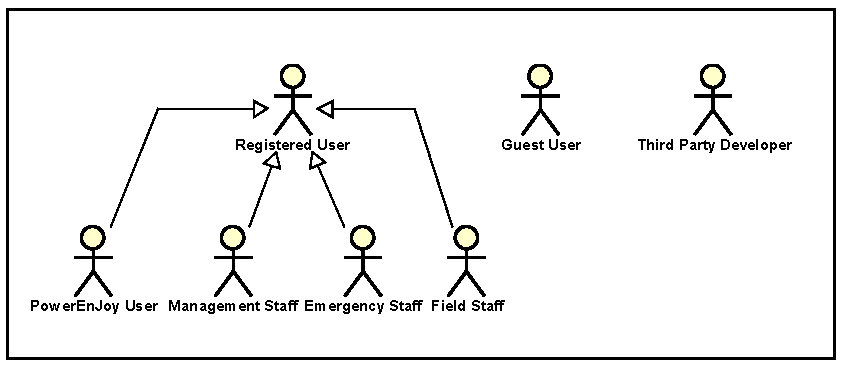
\includegraphics[scale=0.85]{Actors.pdf} }\\
	Here we explain which is the hierarchy of users. See Users definitions in the \hyperref[sec:Glossary]{Glossary}.  
	\subsection{Use Cases}
		\subsubsection{Registration}
		\begin{center}
		\begin{tabular}{l||p{10cm}}
		\textbf{Name} 
			& Registration\\ [8px]
		\textbf{Actors} 
			& Guest user\\ [8px]
		\textbf{Assumptions} 
			& \begin{itemize}
				\item The guest downloaded the app.
			\end{itemize}\\
		\textbf{Flow of events}
			& \begin{enumerate}
	 			\item The user opens PowerEnJoy app on his smartphone.
				\item The guest provides his credentials and documents to the system.
				\item The system verify user's credentials and documents to ensure that he can register in.
				\item The system sends to the user's e-mail address his own password and pin.
			\end{enumerate}\\ 
		\textbf{Exit conditions}
			& The guest has become a registered user.\\ [8px]
		\textbf{Exceptions}
			& \begin{itemize}
				\item The user's credentials are unsuccessfully verified, an error message is shown. The user is not registered.
			\end{itemize}
		\end{tabular}
		\end{center}
	
		\noindent
		\makebox[\textwidth]{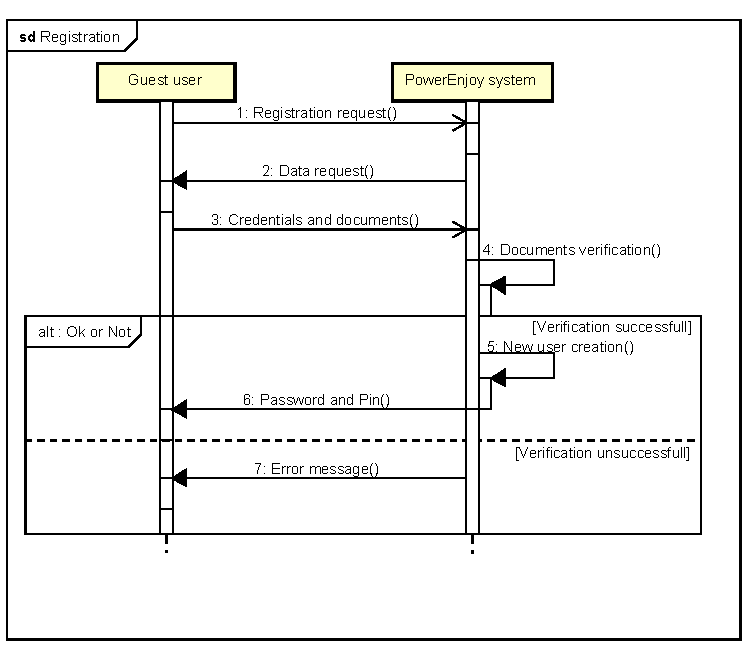
\includegraphics[scale=0.85]{Registration.pdf} }%


		\subsubsection{Credentials and Documents Verification}
		\begin{center}
		\begin{tabular}{l||p{10cm}}
		\textbf{Name} 
			& Credentials and documents verification\\ [8px]
		\textbf{Actors} 
			& Bank system, Motorization system\\ [8px]
		\textbf{Assumptions} 
			& \begin{itemize}
				\item The system owns user's documents.
			\end{itemize}\\
		\textbf{Flow of events}
			& \begin{enumerate}
	 			\item The system sends the documents to the competence authorities.
				\item The authorities check the authenticity of the documents.
				\item The authorities send the confirmation to the system.
			\end{enumerate}\\ 
		\textbf{Exit conditions}
			& The user's documents are authenticated.\\ [8px]
		\textbf{Exceptions}
			& \begin{itemize}
				\item The system receives a negative reply from at least one authority. The verification is rejected.
			\end{itemize}
		\end{tabular}
		\end{center}
		\noindent
		\makebox[\textwidth]{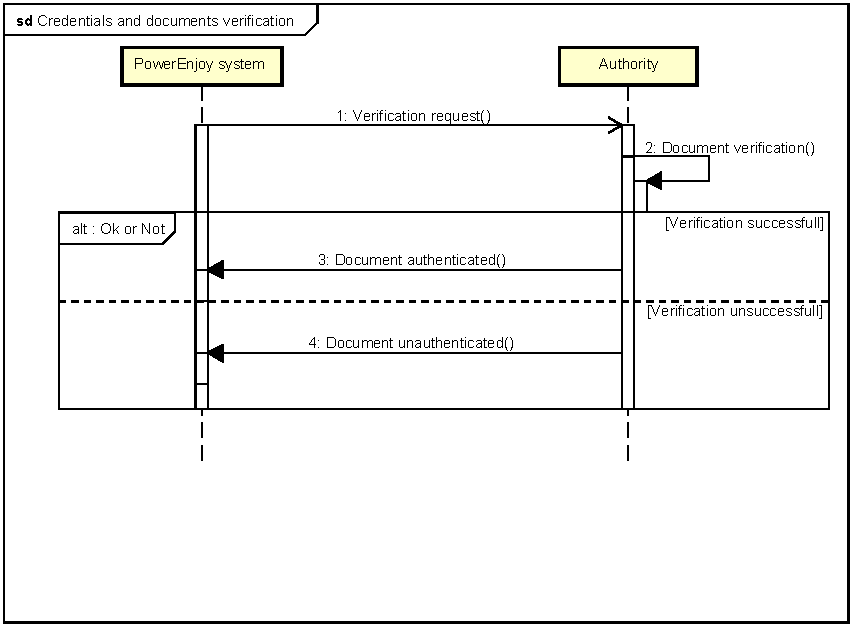
\includegraphics[scale=0.85]{Credentials_and_documents_verification.pdf}}%


		\subsubsection{Login}
		\begin{center}
		\begin{tabular}{l||p{10cm}}
		\textbf{Name} 
			& Login\\ [8px]
		\textbf{Actors} 
			& Registered user\\ [8px]
		\textbf{Assumptions} 
			& \begin{itemize}
				\item The user has successfully signed up to the system.
				\item The user is not logged to the system yet.
			\end{itemize}\\
		\textbf{Flow of events}
			& \begin{enumerate}
	 			\item The user opens the app.
				\item The user declares his identity.
				\item The system recognises the identity and ensures that the user who is logging in is who he claims to be.
				\item The user can visualize his personal page and access to system's functionalities provided to him.
			\end{enumerate}\\ 
		\textbf{Exit conditions}
			& The user is logged into the system now.\\ [8px]
		\textbf{Exceptions}
			& \begin{itemize}
				\item The informations inserted are wrong, an error message is shown. The user is not logged.
			\end{itemize}
		\end{tabular}
		\end{center}
		\noindent
		\makebox[\textwidth]{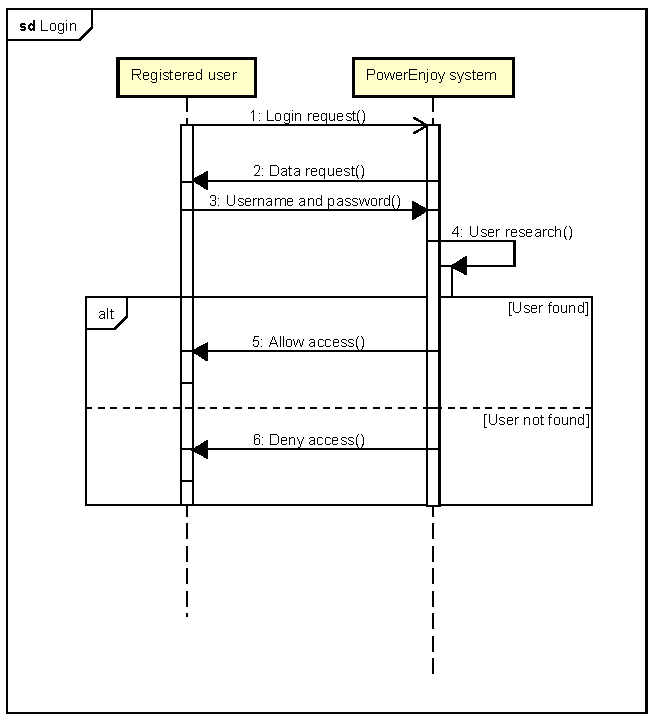
\includegraphics[scale=0.85]{Login.pdf}}%

		\subsubsection{Password Recovery}
		\begin{center}
		\begin{tabular}{l||p{10cm}}
		\textbf{Name} 
			& Password recovery\\ [8px]
		\textbf{Actors} 
			& Registered user\\ [8px]
		\textbf{Assumptions} 
			& \begin{itemize}
				\item The user is not logged to the system yet.
			\end{itemize}\\
		\textbf{Flow of events}
			& \begin{enumerate}
	 			\item The user opens the app.
				\item The user selects the recovery password option.
				\item The user provides to the system his own pin and e-mail address.
				\item The system checks that the pin and the address inserted are associated.
				\item The system sends an e-mail containing the forgotten password to the user's e-mail address.
			\end{enumerate}\\ 
		\textbf{Exit conditions}
			& The e-mail containing the password is sent.\\ [8px]
		\textbf{Exceptions}
			& \begin{itemize}
				\item The pin and address inserted are not associated, an error message is shown. The e-mail is not sent.
			\end{itemize}
		\end{tabular}
		\end{center}
		\noindent
		\makebox[\textwidth]{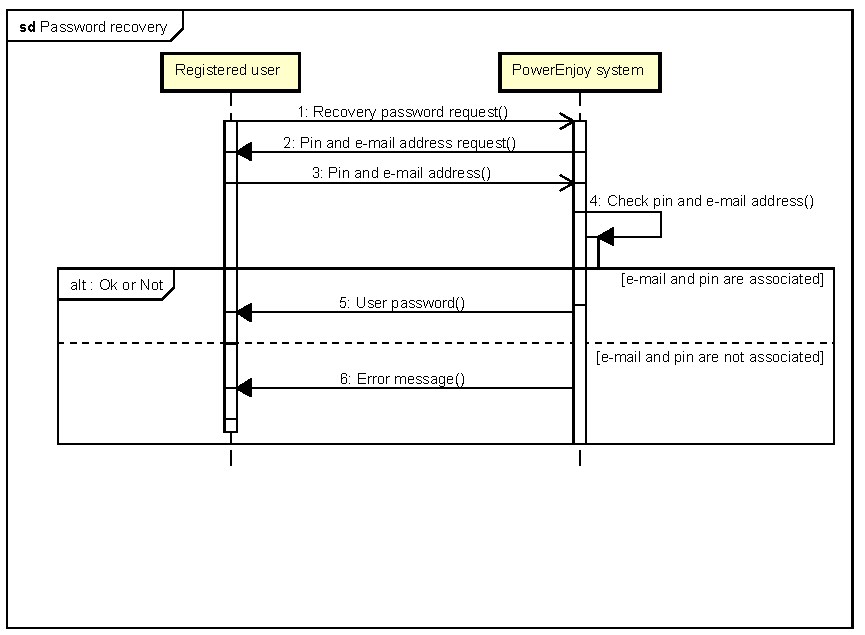
\includegraphics[scale=0.85]{Password_recovery.pdf}}%

		\subsubsection{Update Safe Areas}
		\begin{center}
		\begin{tabular}{l||p{10cm}}
		\textbf{Name} 
			& Update safe areas\\ [8px]
		\textbf{Actors} 
			& Management staff\\ [8px]
		\textbf{Assumptions} 
			& \begin{itemize}
				\item The user is logged as management staff to the system yet.
			\end{itemize}\\
		\textbf{Flow of events}
			& \begin{enumerate}
	 			\item The staff goes in the safe area section of the app, that is visible only by management staff.
				\item The user interface shows a list of actual safe areas.
				\item The staff select to add a new safe area or to update an existing one.
				\item The staff provides the necessary parameters for the action.
				\item The system takes care of the request.
			\end{enumerate}\\ 
		\textbf{Exit conditions}
			& The safe areas set is updated.\\ [8px]
		\textbf{Exceptions}
			& \begin{itemize}
				\item The parameters inserted are inconsistent, an error message is shown. The safe areas set is unchanged.
			\end{itemize}
		\end{tabular}
		\end{center}
		\noindent
		\makebox[\textwidth]{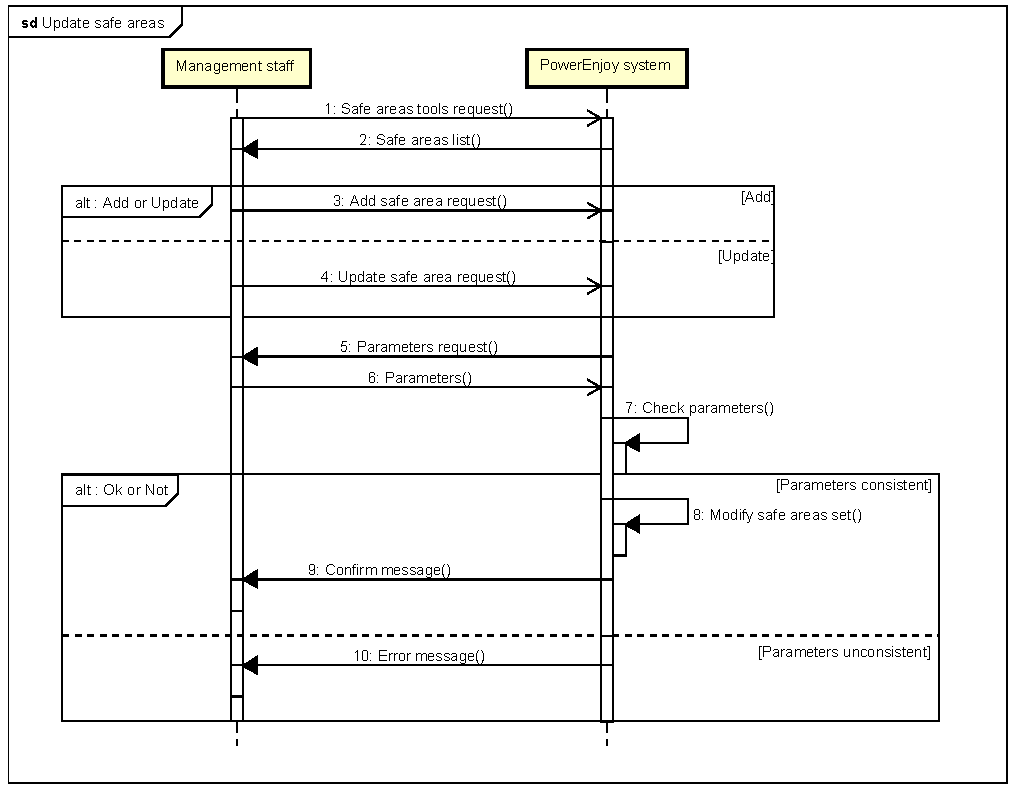
\includegraphics[scale=0.85]{Update_safe_areas.pdf}}%

		\subsubsection{Update Polices}
		\begin{center}
		\begin{tabular}{l||p{10cm}}
		\textbf{Name} 
			& Update polices\\ [8px]
		\textbf{Actors} 
			& Management staff\\ [8px]
		\textbf{Assumptions} 
			& \begin{itemize}
				\item The user is logged as management staff to the system yet.
			\end{itemize}\\
		\textbf{Flow of events}
			& \begin{enumerate}
	 			\item The staff goes in the polices section of the app, that is visible only by management staff.
				\item The user interface shows a list of actual polices.
				\item The staff select to add a new policy or to update an existing one.
				\item The staff provides the necessary parameters for the action.
				\item The system notify the users that the policies are changed and it blocks them account until they accept the new policies.
			\end{enumerate}\\ 
		\textbf{Exit conditions}
			& The policies set is updated.\\ [8px]
		\textbf{Exceptions}
			& \begin{itemize}
				\item The parameters inserted are inconsistent, an error message is shown. The policies set is unchanged.
			\end{itemize}
		\end{tabular}
		\end{center}
		\noindent
		\makebox[\textwidth]{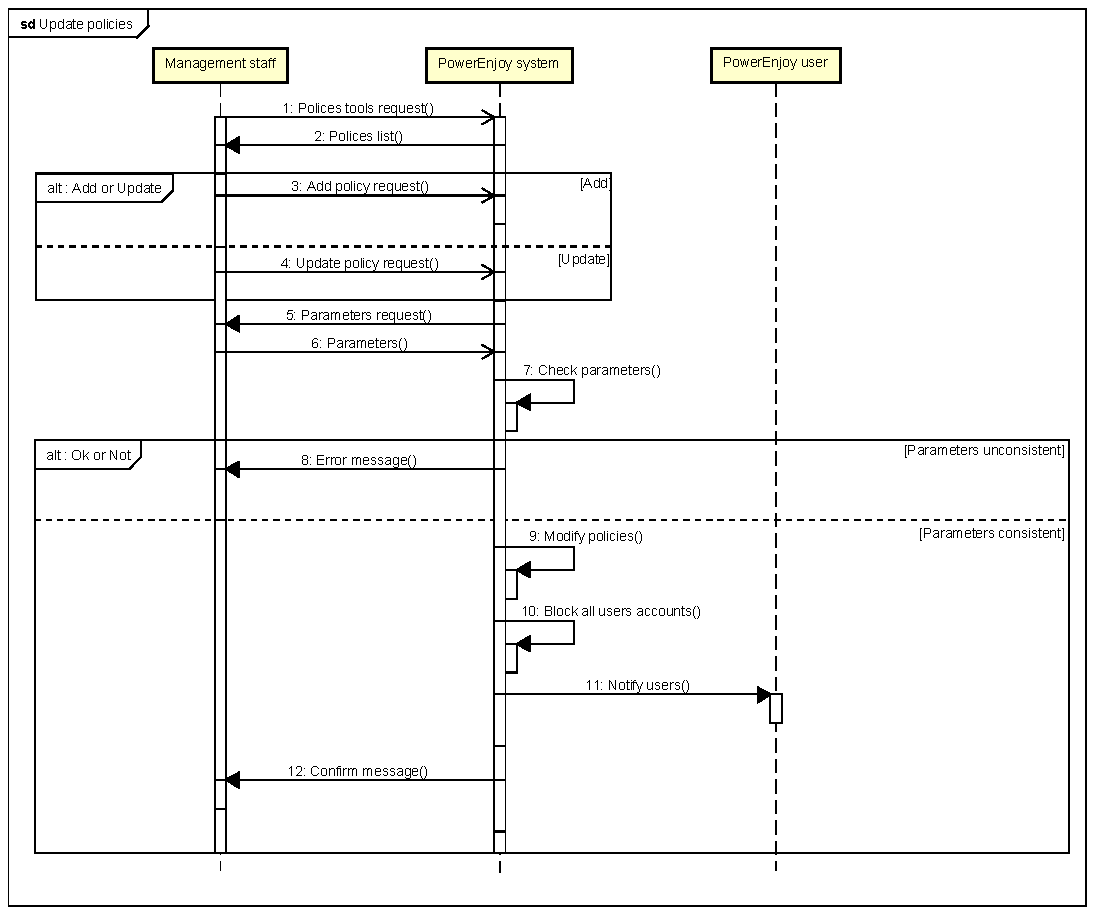
\includegraphics[scale=0.85]{Update_policies.pdf}}%

		\subsubsection{Notify Users}
		\begin{center}
		\begin{tabular}{l||p{10cm}}
		\textbf{Name} 
			& Notify users\\ [8px]
		\textbf{Actors} 
			& PowerEnjoy user\\ [8px]
		\textbf{Assumptions} 
			& \begin{itemize}
				\item The user is logged to the system yet.
			\end{itemize}\\
		\textbf{Flow of events}
			& \begin{enumerate}
	 			\item The user interface shows a message informing the user that the policies are changed.
				\item The user accepts the new conditions. 
				\item The system unlock his account.
			\end{enumerate}\\ 
		\textbf{Exit conditions}
			& Will be applied the new policies to the user.\\ [8px]
		\textbf{Exceptions}
			& \begin{itemize}
				\item The user doesn't accept the new conditions. The user's account is deleted.
			\end{itemize}
		\end{tabular}
		\end{center}

	\subsubsection{Search Car}
	\begin{center}
	\begin{tabular}{l||p{10cm}}
	\textbf{Name} 
		& Search Car\\ [8px]
	\textbf{Actors} 
		& PowerEnJoy User\\ [8px]
	\textbf{Assumptions} 
		& \begin{itemize}
			\item The user is logged in to the system.
		\end{itemize}\\
	\textbf{Flow of events}
		& \begin{enumerate}
	 		\item The user opens PowerEnJoy app on his smartphone 
	 		\item The user interface displays all available cars around the user position according to the setted range. 
			\item Optionally the user can search the cars around an inserted address, or near a remarkable place. 
		\end{enumerate}\\ 
	\textbf{Exit conditions}
		&The user finds a car that satisfies his need and chooses too reserve it.\\ [8px]
	\textbf{Exceptions}
		& \begin{itemize}
			\item The user does not find an useful car and exit the application.
			\item The user want not really reserve a car. 
		\end{itemize}
	\end{tabular}
	\end{center}

	\subsubsection{Reserve Car}
	\begin{center}
	\begin{tabular}{l||p{10cm}}
	\textbf{Name} 
		& Reserve Car\\ [8px]
	\textbf{Actors} 
		& PowerEnJoy User\\ [8px]
	\textbf{Assumptions} 
		& \begin{itemize}
			\item The user is logged in to the system.
			\item The user has Searched Cars and has find an optimal one
		\end{itemize}\\
	\textbf{Flow of events}
		& \begin{enumerate}
 			\item The user selects the car that he want reserve
 			\item The user interface displays all informations about the car (E.g. Autonomy in km) and a button for reserve it. 
			\item The user chooses to reserve the car. 
			\item The user confirms his choose.
		\end{enumerate}\\ 
	\textbf{Exit conditions}
		&The system confirms the successful reservation, displays the time before reservation expiration and the route for reach it from the current position of the user.\\ [8px]
	\textbf{Exceptions}
		& \begin{itemize}
			\item Reservation expires.
			\item The user exits the procedure before confirming it.
			\item Another user reserves another car while our user is reserving it, the system notify the user. The reservation ends unsuccessfully.
		\end{itemize}
	\end{tabular}
	\end{center}

	\subsubsection{Cancel Reservation}
	\begin{center}
	\begin{tabular}{l||p{10cm}}
	\textbf{Name} 
		& Cancel Reservation\\ [8px]
	\textbf{Actors} 
		& PowerEnJoy User\\ [8px]
	\textbf{Assumptions} 
		& \begin{itemize}
			\item The user is logged in to the system.
			\item The user has an active reservation.
		\end{itemize}\\
	\textbf{Flow of events}
		& \begin{enumerate}
 			\item The user opens PowerEnJoy app on his smartphone 
 			\item The user interface displays user's current reservation.
			\item The user eliminates the reservation clicking on the cancel reservation button.
			\item The user confirms his selection.
		\end{enumerate}\\ 
	\textbf{Exit conditions}
		&The user successfully cancel his reservation. The reserved car returns available for other users.\\ [8px]
	\textbf{Exceptions}
		&...\\[8px]
	\end{tabular}
	\end{center}

	\subsubsection{Pick up car}
	\begin{center}
	\begin{tabular}{l||p{10cm}}
	\textbf{Name} 
		& Pick up car\\ [8px]
	\textbf{Actors} 
		& PowerEnJoy User\\ [8px]
	\textbf{Assumptions} 
	& \begin{itemize}
		\item The user is logged in to the system.
		\item The user has a reservation active.
		\item The user is no far than 10 meters from the car.
		\item The user inserts the correct \personalpin 
	\end{itemize}\\
	\textbf{Flow of events}
		& \begin{enumerate}
 		\item The user is close to his reserved car.
 		\item The user selects the unlock car button (displayed in the application) UI on it's smartphone.
		\item The system unlocks the car.
		\item The user gets in the car and insets his \personalpin.
		\item The system detects all passengers from cars sensors.
		\item Driving command are enabled by the system. 
		\item Optionally the user can decide to activate the "Money Saving Option".
		\item The user starts driving his car.
		\item the system calculates the fare and shows it on the display.
		\end{enumerate}\\ 
	\textbf{Exit conditions}
		&\begin{itemize}
			\item The user makes a \stopover.
			\item The user releases car.
		\end{itemize}\\
	\textbf{Exceptions}
		& \begin{itemize}
			\item The user run out of money on his credit card.
			\item The car runs out of battery.
		\end{itemize}
	\end{tabular}
	\end{center}
	
	\subsubsection{Stand}
	\begin{center}
	\begin{tabular}{l||p{10cm}}
	\textbf{Name} 
		& Stand\\ [8px]
	\textbf{Actors} 
		& PowerEnJoy User\\ [8px]
	\textbf{Assumptions} 
	& \begin{itemize}
		\item The user has picked up a car. 
	\end{itemize}\\
	\textbf{Flow of events}
		& \begin{enumerate}
 		\item The user parks the car.
 		\item The user selects the \stopover option on the car screen.
		\item Driving command are disabled by the system. 
		\item The user get off the car.
		\item The system locks the car.
		\end{enumerate}\\ 
	\textbf{Exit conditions}
		&\begin{itemize}
			\item When the user wants end the \stopover he re-unlocks and start driving the car as he has done in the "Pick up car" use case.
		\end{itemize}\\
	\textbf{Exceptions}
		& \begin{itemize}
			\item The user run out of money on his credit card. (The user will not be able to re-unlock the car.)
		\end{itemize}
	\end{tabular}
	\end{center}
	
	\subsubsection{Money Saving Option}
	\begin{center}
	\begin{tabular}{l||p{10cm}}
	\textbf{Name} 
		& Money Saving Option\\ [8px]
	\textbf{Actors} 
		& PowerEnJoy User\\ [8px]
	\textbf{Assumptions} 
	& \begin{itemize}
		\item The user has picked up a car. 
	\end{itemize}\\
	\textbf{Flow of events}
		& \begin{enumerate}
 		\item The user selects his destination address on the car screen
		\item The system purposes the \powergrid station according to algorithm constraints.
		\end{enumerate}\\ 
	\textbf{Exit conditions}
		&\begin{itemize}
			\item The user releases the car.
		\end{itemize}\\
	\textbf{Exceptions}
		& \begin{itemize}
			\item There are no available \powergrid stations in 1 km range from the destination. (The system during driving will notify the user through the car screen if a \powergrid becomes free.)
		\end{itemize}
	\end{tabular}
	\end{center}

	\subsubsection{Release Car}
	\begin{center}
	\begin{tabular}{l||p{10cm}}
	\textbf{Name} 
		& Release Car\\ [8px]
	\textbf{Actors} 
		& PowerEnJoy User\\ [8px]
	\textbf{Assumptions} 
	& \begin{itemize}
		\item The user has picked up a car. 
	\end{itemize}\\
	\textbf{Flow of events}
		& \begin{enumerate}
 		\item The user parks the car in a \safearea.
		\item The user selects the end \carsharing option on the car screen.
		\item Driving command are disabled by the system. 
		\item The system starts calculating fare discounts.
		\end{enumerate}\\ 
	\textbf{Exit conditions}
		&\begin{itemize}
			\item The user get off the car, than the system locks the car.
		\end{itemize}\\
	\textbf{Exceptions}
		& \begin{itemize}
			\item The user is not in a safe area and he cannot end \carsharing. 
		\end{itemize}
	\end{tabular}
	\end{center}

\subsubsection{Plug car}
	\begin{center}
	\begin{tabular}{l||p{10cm}}
	\textbf{Name} 
		& Plug Car\\ [8px]
	\textbf{Actors} 
		& PowerEnJoy User\\ [8px]
	\textbf{Assumptions} 
	& \begin{itemize}
		\item The user has parked a car near a \powergrid and has ended his \carsharing. 
	\end{itemize}\\
	\textbf{Flow of events}
		& \begin{enumerate}
 			\item The user inserts his \personalpin into the \powergrid screen, in order to let the \powergrid enabled to charge cars.
			\item The user plugs the car to the \powergrid.
			\item The system detects that the car of our user is charging at the \powergrid unlocked by the same user. 
		\end{enumerate}\\ 
	\textbf{Exit conditions}
		&\begin{itemize}
			\item The user receives the expected discount.
		\end{itemize}\\
	\textbf{Exceptions}
		&...\\[8px]
	\end{tabular}
	\end{center}

\subsubsection{Handle Emergency}
	\begin{center}
	\begin{tabular}{l||p{10cm}}
	\textbf{Name} 
		& Handle Emergency\\ [8px]
	\textbf{Actors} 
		& Emergency Staff, PowerEnJoy User\\ [8px]
	\textbf{Assumptions} 
		&...\\[8px]
	\textbf{Flow of events}
		& \begin{enumerate}
			\item The system notifies the Emergency Staff that an emergency rose up.
			\item Given the nature of the emergency the staff handles.
				\begin{itemize}
					\item if the emergency is a "Help Request" the staff is able to interact to the \powerenjoyuser.
					\item if a "Car Accident" has happened the staff takes the proper decisions, and the field staff is alerted.
					\item if a car has the "Empty Battery" the Emergency Staff signals it to the Field Staff.
			\end{itemize} 
		\end{enumerate}\\ 
	\textbf{Exit conditions}
		&\begin{itemize}
			\item The emergency has been resolved.
		\end{itemize}\\
	\textbf{Exceptions}
		&...\\[8px]
	\end{tabular}
	\end{center}

\subsubsection{Maintain Car}
	\begin{center}
	\begin{tabular}{l||p{10cm}}
	\textbf{Name} 
		&Maintain Car\\ [8px]
	\textbf{Actors} 
		& Field Staff\\ [8px]
	\textbf{Assumptions} 
		&An issue with a car has happened.\\
	\textbf{Flow of events}
		& \begin{enumerate}
			\item The Field Staff reaches the car that needs maintenance.
			\item The Field Staff evaluates the car situation and take a decision on how to maintain it. 
			\item Once the car is repaired the field staff relocates the car in a \safearea and set it visible to PowerEnJoy Users.
		\end{enumerate}\\ 
	\textbf{Exit conditions}
		&\begin{itemize}
			\item The car has been maintained.
		\end{itemize}\\
	\textbf{Exceptions}
		&The car cannot be maintained.\\[8px]
	\end{tabular}
	\end{center}

	\subsection{Class Diagram}
\section{External Interfaces}
In order to deploy our system, given Goals, Domain Assumptions and Requirements, we would like to give a boundary of the hardware and external software systems that will be involved in our project.
\subsection{User Devices}
	Each \powerenjoyuser, and \fieldstaff user should operate through a device that has these characteristics:
		\begin{itemize}
			\item Network connection
			\item Geolocation system capable to give a precision comparable to the one given by the GPS used for civil scopes.
		\end{itemize}
\subsection{Cars}
	Each Car used for the \powerenjoy service must be equipped with these features:
	\begin{itemize}
		\item Touch Screen
		\item Speakerphone
		\item Occupant classification system
		\item Geolocation system
		\item on-board computer supporting the chosen Navigation system
		\item Network connection
		\item ECU (Electronic Control Unit) must be able to supervise the car needs of maintenance via specific sensors (e.g. tire pressure sensor)
		\end{itemize}
	Furthermore the battery autonomy that is displayed to the \powerenjoyuser is rescaled to map real 10-100\% to 0-100\%.
	\begin{figure}[H]
\centering
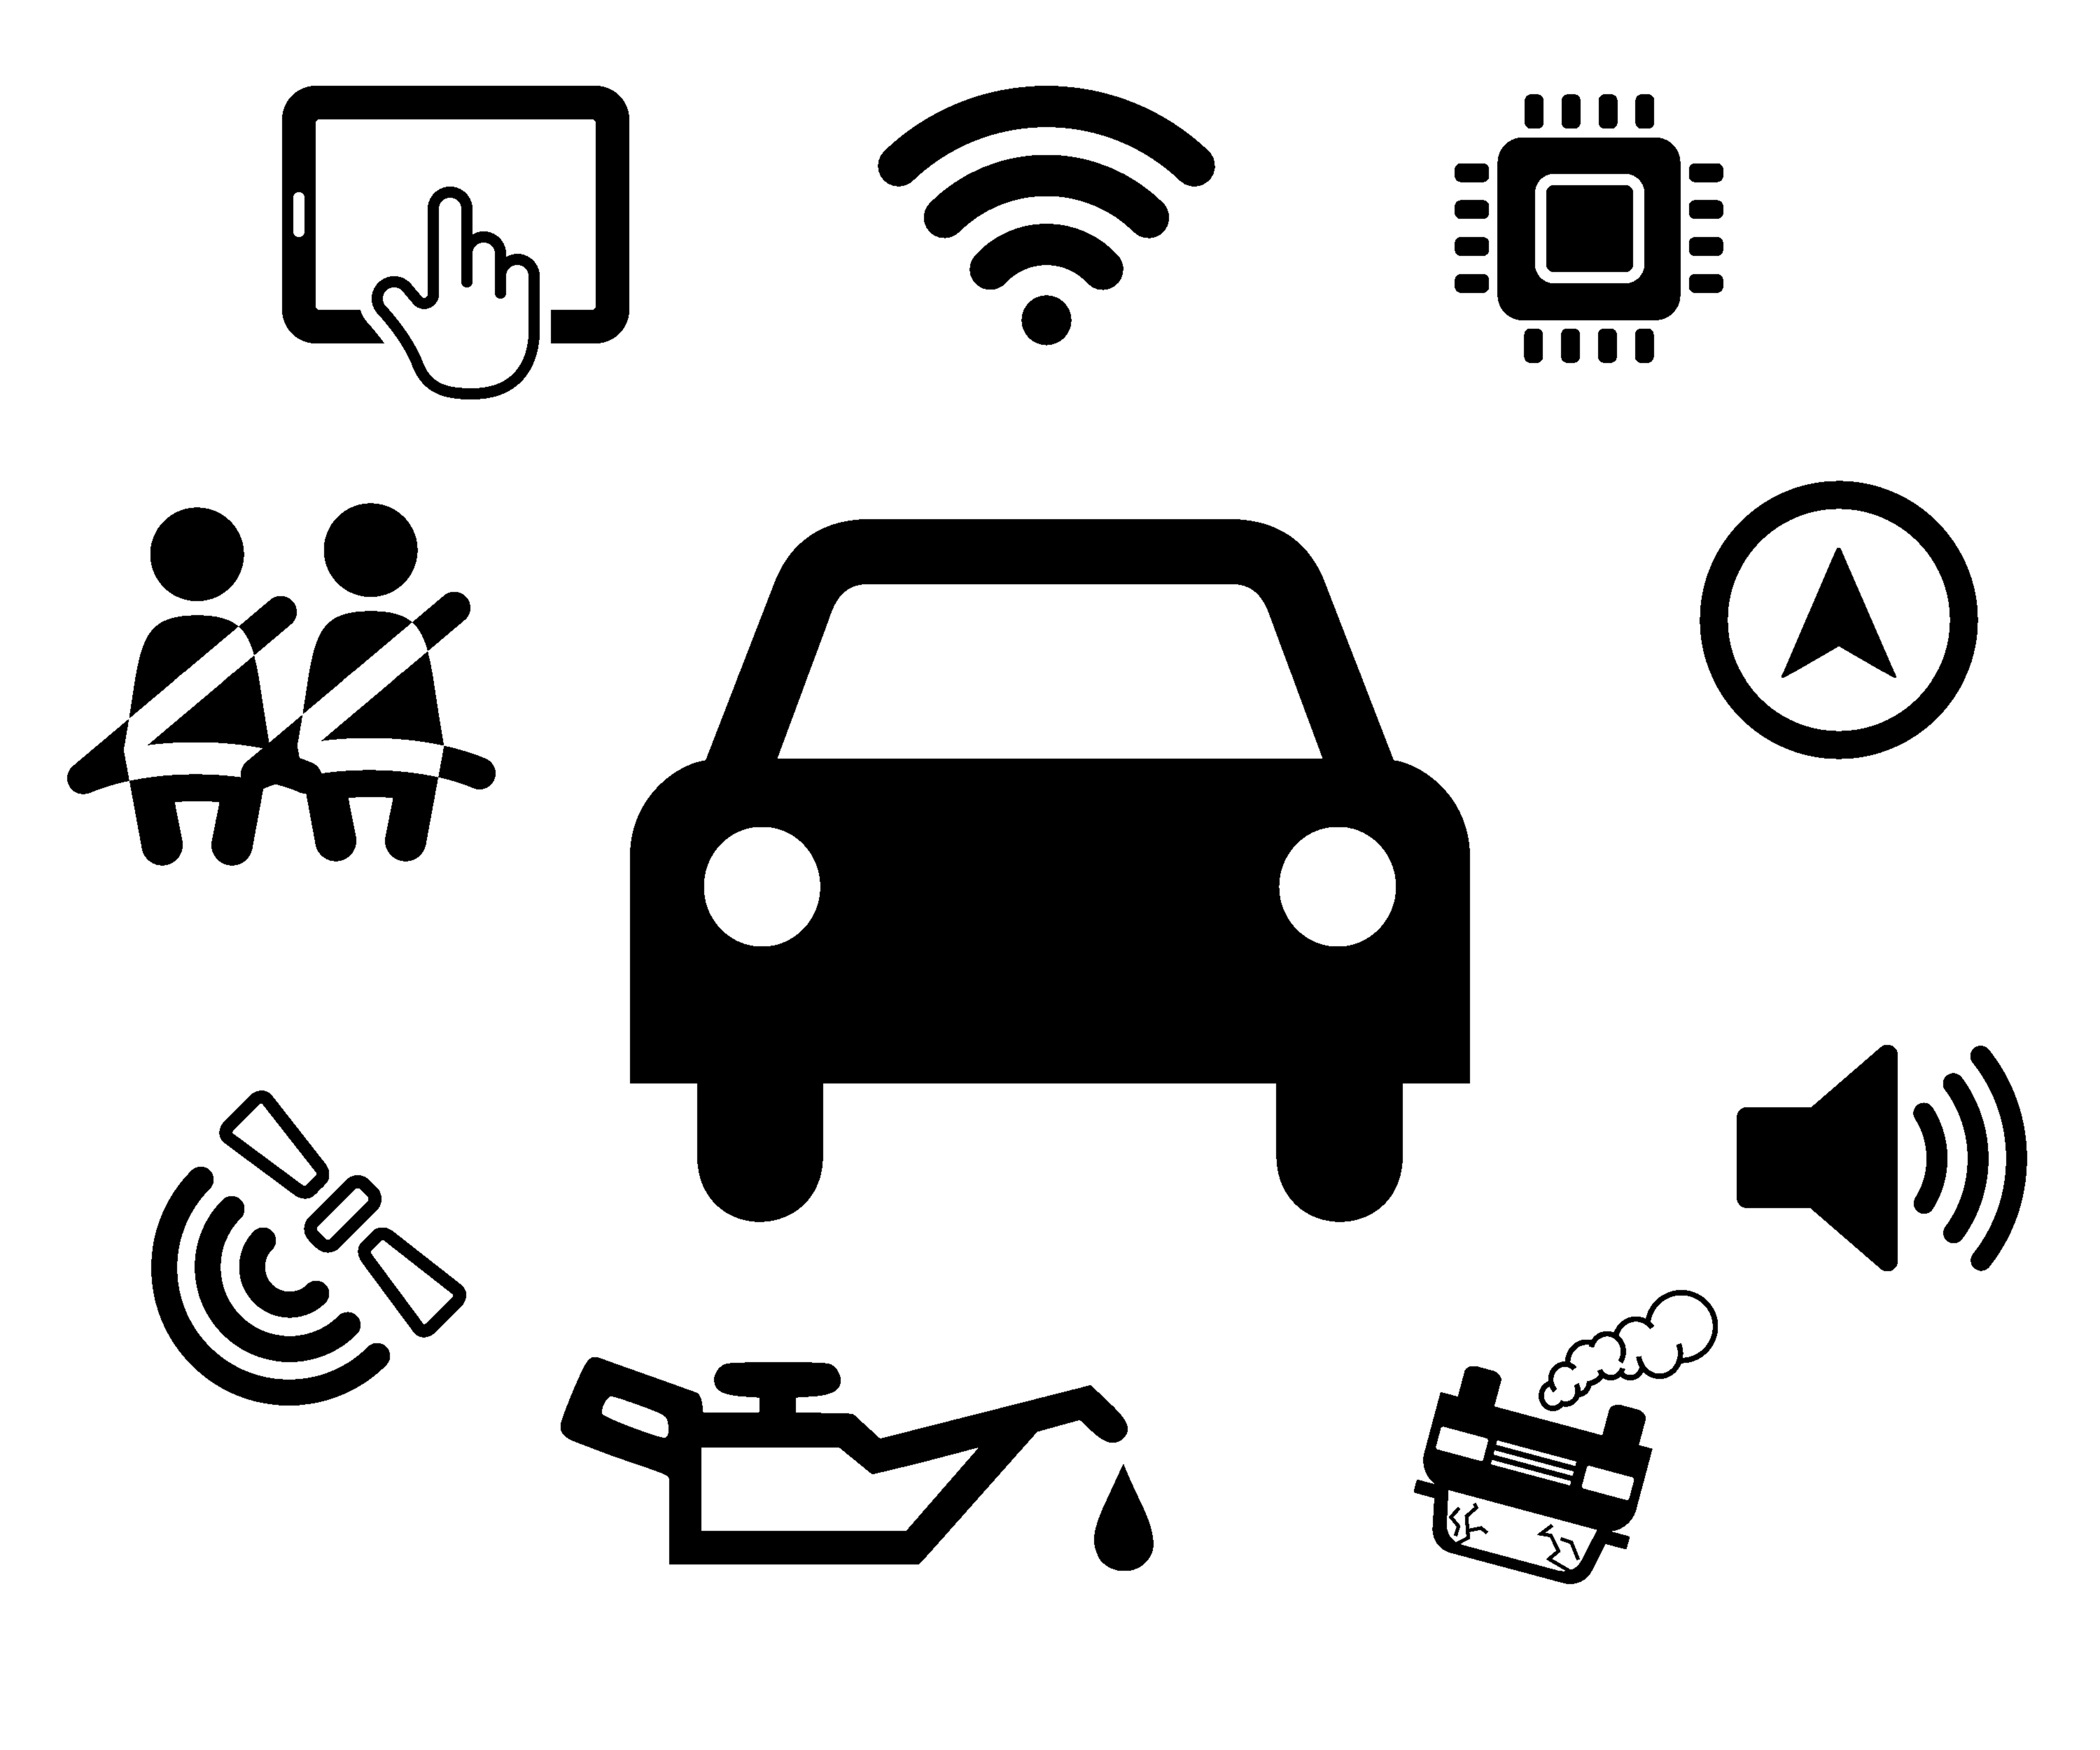
\includegraphics[scale=0.1]{auto.pdf}% "%" necessario

\caption{City Zones Map division}
\end{figure}

		
\subsection{Power Plug}
	Each power plug for the \powerenjoy service must be equipped as follow:
		\begin{itemize}
			\item Network Connection
			\item Phisical/Touch keyboard in order to allow \personalpin insertion.
		\end{itemize}
\subsection{Navigation System}
	The navigation and map system will be provided from an external services through their API (e.g. TomTom, Google Maps).
\subsection{Payments}
	The payments system will be provided by external services through their API (e.g.Stripe, Dwolla).

\section{Alloy Model}
	
	\lstinputlisting[language=alloy, frame=trBL, caption=Complete Alloy Code]{Alloy.als}
	

\section{Hours of Work}

\end{document}